
%(BEGIN_QUESTION)
% Copyright 2011, Tony R. Kuphaldt, released under the Creative Commons Attribution License (v 1.0)
% This means you may do almost anything with this work of mine, so long as you give me proper credit

\noindent
{\bf Programming Challenge and Comparison -- Batch mixing sequence control} 

\vskip 10pt

Tony loves garlic-infused olive oil, and so he decides to build an automated process for mixing large batches of it:

$$\includegraphics[width=15.5cm]{i03836x01.eps}$$

\vskip 10pt

Write a PLC program to perform the following sequence, each step lasting 5 seconds (to make testing the program easier):

% No blank lines allowed between lines of an \halign structure!
% I use comments (%) instead, so that TeX doesn't choke.

$$\vbox{\offinterlineskip
\halign{\strut
\vrule \quad\hfil # \ \hfil & 
\vrule \quad\hfil # \ \hfil & 
\vrule \quad\hfil # \ \hfil & 
\vrule \quad\hfil # \ \hfil & 
\vrule \quad\hfil # \ \hfil & 
\vrule \quad\hfil # \ \hfil \vrule \cr
\noalign{\hrule}
%
% First row
{\bf Step} & {\bf Action} & Oil valve & Mixer motor & Garlic feed & Drain valve \cr
%
\noalign{\hrule}
%
% Another row
1 & Drain valve off, oil valve on & on & off & off & off \cr
%
\noalign{\hrule}
%
% Another row
2 & Oil valve off, mixer on & off & on & off & off \cr
%
\noalign{\hrule}
%
% Another row
3 & Garlic feed on & off & on & on & off \cr
%
\noalign{\hrule}
%
% Another row
4 & Garlic feed off & off & on & off & off \cr
%
\noalign{\hrule}
%
% Another row
5 & Mixer off, drain valve on & off & off & off & on \cr
%
\noalign{\hrule}
} % End of \halign 
}$$ % End of \vbox

\begin{itemize}
\item{} {\bf Inputs} 
\item{} Start pushbutton (momentary NO) -- {\it press to begin the mixing sequence}
\item{} Stop pushbutton (momentary NO) -- {\it press to halt (freeze) the mixing sequence}
\item{} Reset pushbutton (momentary NO) -- {\it press to reset the sequence to the first step}
\end{itemize}

\begin{itemize}
\item{} {\bf Outputs} 
\item{} Oil valve -- {\it energize to open up the oil valve, admitting oil into the mixing tank}
\item{} Mixer motor -- {\it energize to turn the mixer paddle}
\item{} Garlic feed -- {\it energize to add ground garlic to the mixing tank via the screw conveyor}
\item{} Drain valve -- {\it energize to open up the valve and drain the mixing tank}
\end{itemize}

\filbreak

Write a PLC program performing this function, and demonstrate its operation using switches connected to its inputs to simulate the discrete inputs in a real application.  

\vskip 10pt

When your program is complete and tested, capture a screen-shot of it as it appears on your computer, and prepare to present your program solution to the class in a review session for everyone to see and critique.  The purpose of this review session is to see multiple solutions to one problem, explore different programming techniques, and gain experience interpreting PLC programs others have written.  When presenting your program, prepare to discuss the following points:

\begin{itemize}
\item{} Identify the ``tag names'' or ``nicknames'' used within your program to label I/O and other bits in memory
\item{} Follow the sequence of operation in your program, simulating the system in action
\item{} Identify any special or otherwise non-standard instructions used in your program, and explain why you decided to take that approach
\item{} Show the comments placed in your program, to help explain how and why it works
\item{} How you designed the program (i.e. what steps you took to go from a concept to a working program)
\end{itemize}

\underbar{file i03836}
%(END_QUESTION)





%(BEGIN_ANSWER)


%(END_ANSWER)





%(BEGIN_NOTES)

$$\includegraphics[width=15.5cm]{i03836x02.eps}$$

% No blank lines allowed between lines of an \halign structure!
% I use comments (%) instead, so that TeX doesn't choke.

$$\vbox{\offinterlineskip
\halign{\strut
\vrule \quad\hfil # \ \hfil & 
\vrule \quad\hfil # \ \hfil \vrule \cr
\noalign{\hrule}
%
% First row
Register & Contents \cr
%
\noalign{\hrule}
%
% Another row
{\tt B3:1} & 0000000000011000 \cr
%
\noalign{\hrule}
%
% Another row
{\tt B3:2} & 0000000000010100 \cr
%
\noalign{\hrule}
%
% Another row
{\tt B3:3} & 0000000000010110 \cr
%
\noalign{\hrule}
%
% Another row
{\tt B3:4} & 0000000000010100 \cr
%
\noalign{\hrule}
%
% Another row
{\tt B3:5} & 0000000000000001 \cr
%
\noalign{\hrule}
} % End of \halign 
}$$ % End of \vbox

This program simply remains at the last step indefinitely, until the Reset pushbutton is pressed.






\vfil \eject

\noindent
{\bf Summary Quiz:}

(The recommended summary quiz is to have \underbar{each student} demonstrate their PLCs running this particular program)

%INDEX% PLC, programming challenge: batch mixing sequence control
%INDEX% Process: garlic/olive oil mixer

%(END_NOTES)


